\section{Validierung}
Um die Forschungsfragen zu beantworten, haben wir die gesammelten Immobiliendaten auf Verwertbarkeit analysiert und gefiltert.\\
Bei den Machine Learning Algorithmen haben wir den MAPE sowie der MdAPE als wichtiges Performanzkriterium genommen. Weiter war uns wichtig, wie viele Inserate können mit einer Abweichung von 10\% geschätzt werden.\\
Gewisse Daten haben so extreme Werte, dass sie die Diagramme verzerren und so eine Aussage über die Daten erschweren. Deshalb werden diese Werte für die Validation ignoriert. Dabei handelt es sich um insgesamt 751 Inserate. Weiter wurden 12’219 Inserate weggelassen, da bei diesen der Kaufpreis fehlte.
Im nächsten Kapitel wird der Iterative Vorgang beschrieben.
%
\subsection{Gesammelte Daten}
Insgesamt konnten 162’225 Immobilieninserate in einem Zeitraum von 5 Monaten gesammelt werden. Davon stammen die meisten vom Immoscout24 Portal, was in Tabelle \ref{tab:crawled_data} ersichtlich ist.
\begin{table*}[ht]
\centering
\ra{1.3}
\begin{tabular}{@{}lrr@{}}
\toprule
Portal & Anzahl gesammelte Inserate & Anzahl verwendete Inserate \\
\midrule
Immoscout & 94'611 & 46'226\\
Homegate & 34'115 & 19'568\\
Newhome & 32'600 & 19'011\\
Urbanhome & 2'047 & 1'040\\
\bottomrule
\end{tabular}
\caption{Auswertung der gesmmelten Daten}
\label{tab:crawled_data}
\end{table*}
%
Von den insgesamt 162’225 Inseraten wurden 77’608 ungültige Inserate herausgefiltert. 
Dabei handelte es sich mehrheitlich um fehlerhafte Inserate oder Inserate, bei denen wichtige Kennwerte fehlten.\\
Insgesamt konnten 83’107 Wohungen und 65’430 Häuser gesammelt werden. Die restlichen Inserate waren Lagerräume oder nicht definierte Immobilientypen.\\
Weiter konnte für 83\% aller Inserate, mit einer vollständigen Adresse eine Lärmbelastung berechnet werden. Ebenso konnten für 99\% aller Inserate eine Gemeinde zugeordnet werden.\\
Die meisten Inserate haben eine Angabe über die Anzahl Zimmer und Wohnfläche. Gefolgt vom Baujahr und der Anzahl an Stockwerken, falls es mehrere besitzt. Die Raumhöhe oder die Kubatur wird dagegen nur selten angegeben. So auch die effektive Fläche einer Immobilie. Abbildung \ref{fig:features} zeigt den prozentualen Anteil der fehlenden Kennwerte.\\[2ex]
\begin{figure}[h!]
\centering
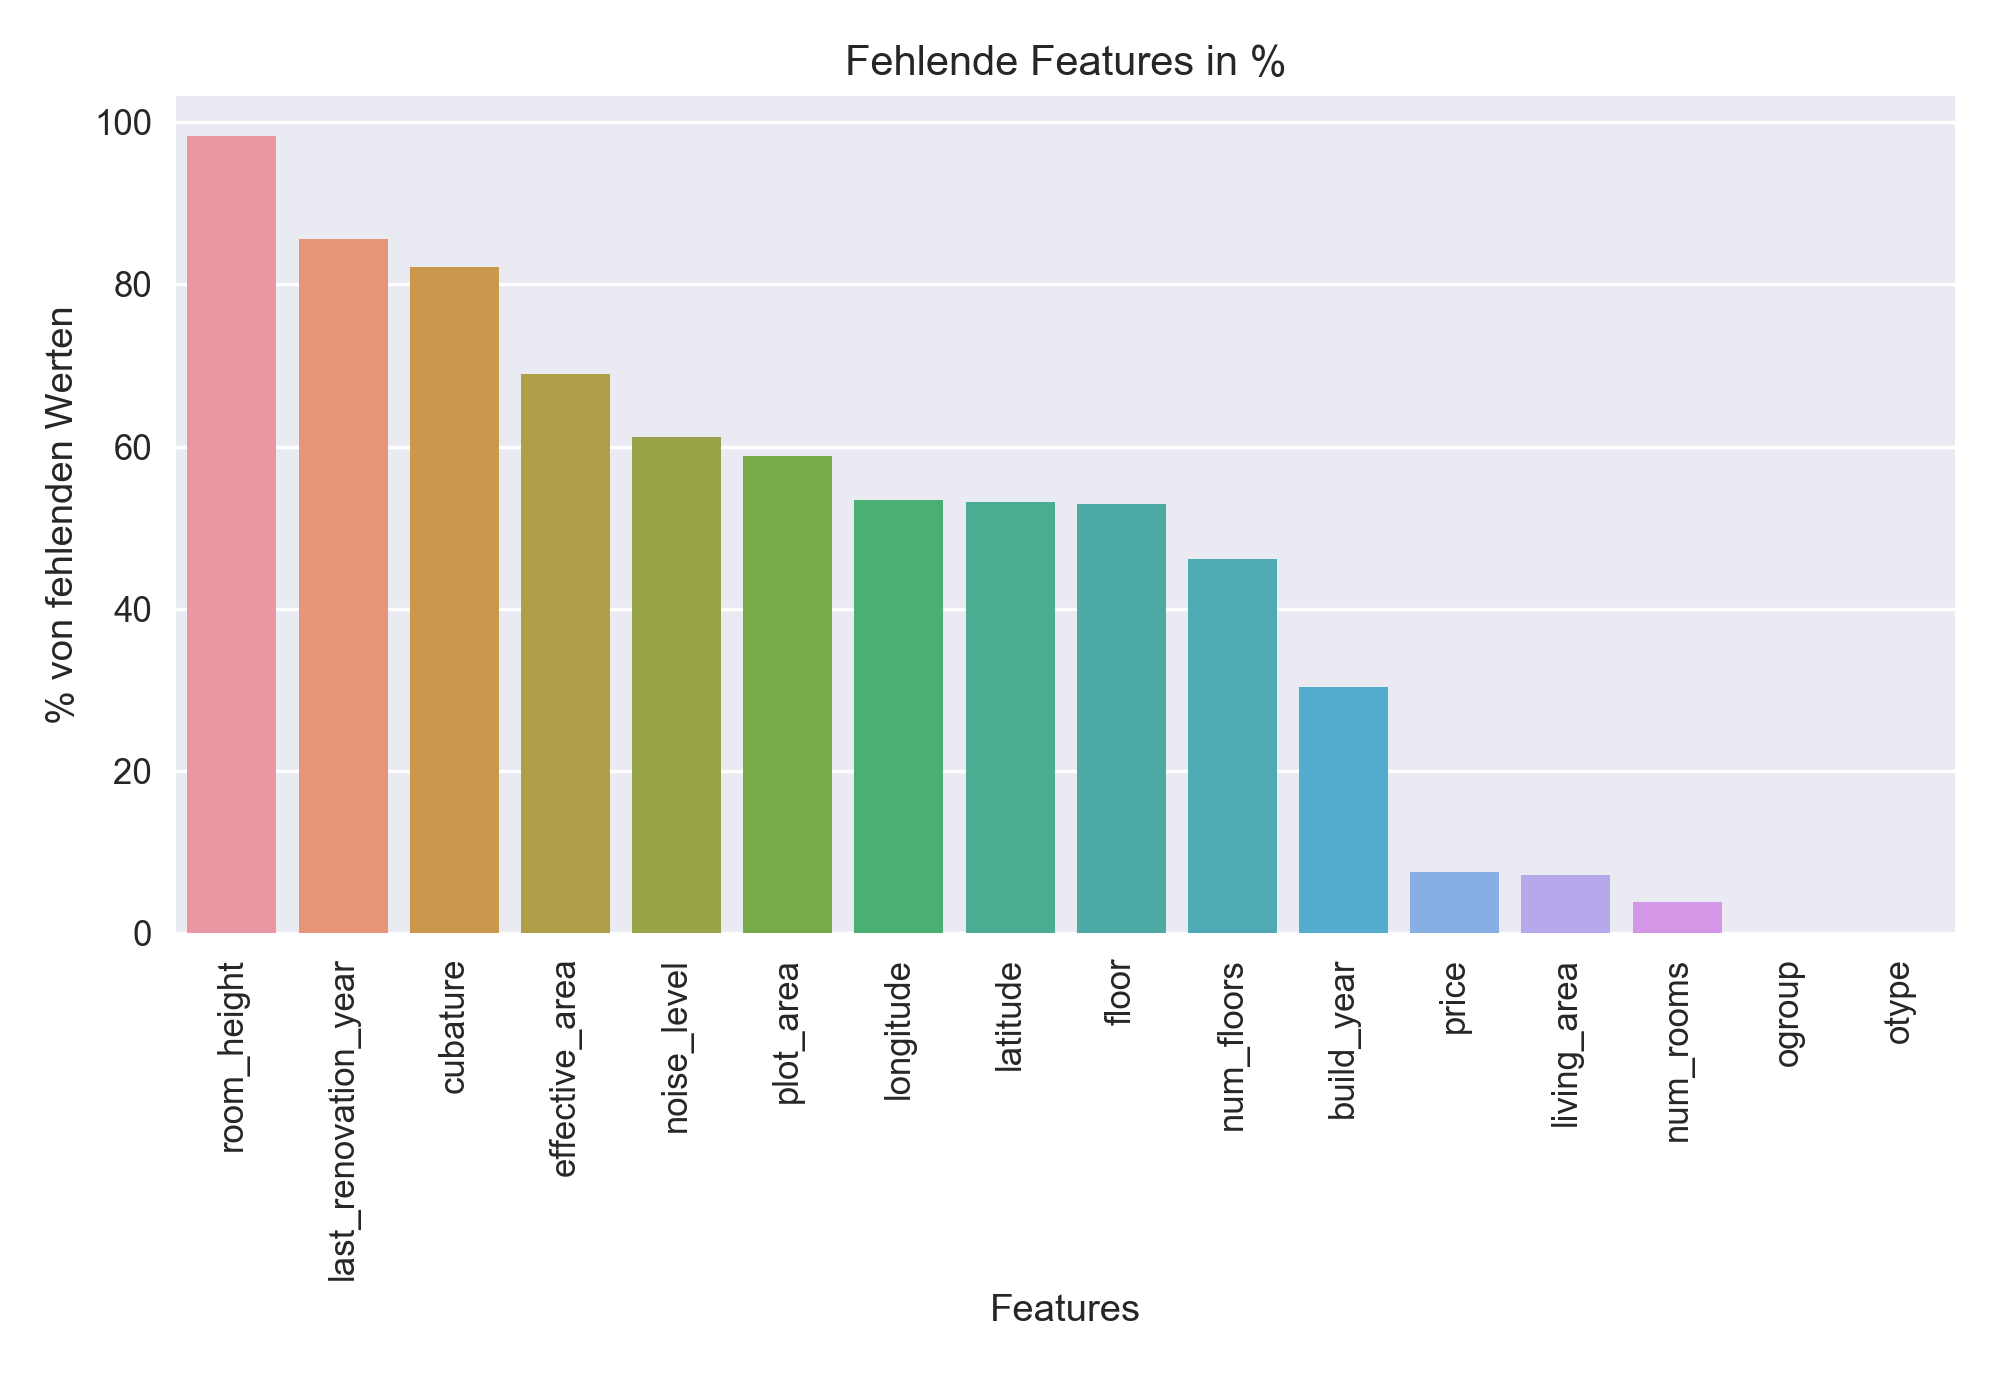
\includegraphics[width=0.9\textwidth]{images/missing_values.png}
\caption[Anzahl der vorkommenden Features]{Anzahl der vorkommenden Features}%
\label{fig:features}
\end{figure}
\newline
%
Die Crawler wurden nie über eine längere Zeit gesperrt. Vereinzelt kam es zu Blockierungen, die jedoch, durch das Starten neuer Proxyinstanzen, umgehen werden konnten. Der Zeitaufwand um ein Portal bei fünf gleichzeitigen Verbindungen und einer Download Delay von zwei Sekunden zu crawlen, lag im Schnitt bei 4 Stunden. Dementsprechend wurden in dieser Zeit etwa 100 Proxyinstanzen gestartet.\\[2ex]
%
Die Datenqualität ist eher mässig, da viele Inserate erst gar nicht für ein Trainingsdatensatz verwendet werden können. Um dem entgegenzuwirken, wurde versucht durch Feature Engineering fehlende Daten zu berechnen.
%
\subsubsection{Kaufpreis}
Abbildung \ref{fig:price} zeigt die Verteilung des Kaufpreises. Dabei sieht man, dass dieser nicht normalverteilt ist (\ref{fig:price_normal}). Es besteht eine positive Skenwess, was für eine Lineare Regression nicht optimal ist. Wird der Log-Wert des Preises genommen (\ref{fig:price_log}), kann eine Annäherung an eine Normalverteilung erreicht werden. Dies gilt es zu beachten, wenn später mit einer Linearen Regression gearbeitet wird.
Tabelle () zeigt die beschreibenden statistischen Werte des Preises.
%
\begin{figure}[ht]
\begin{subfigure}{.5\textwidth}
  \centering
  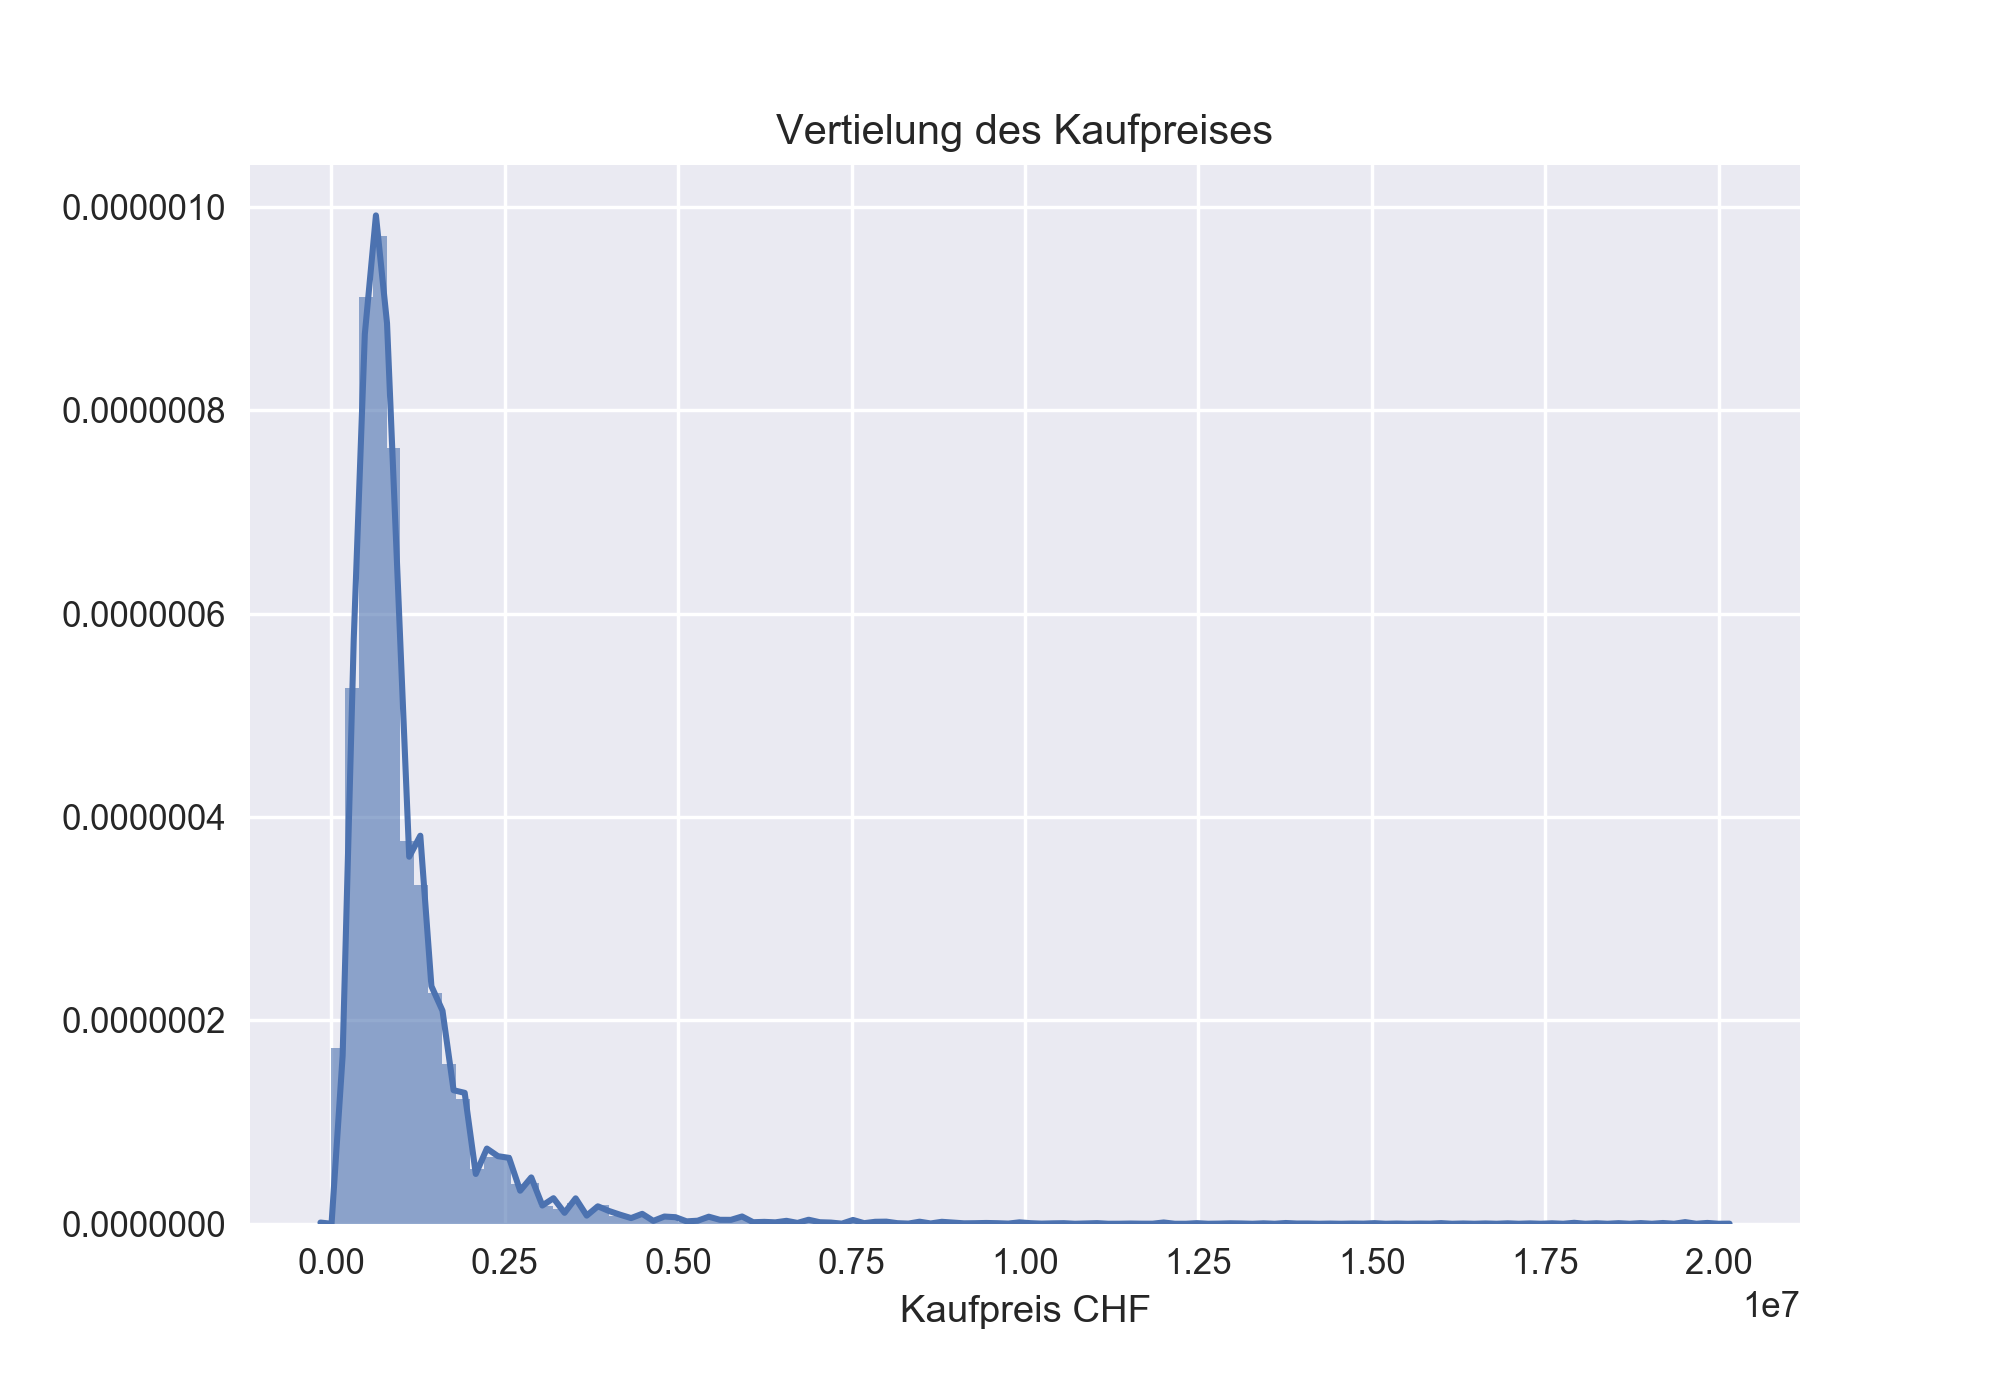
\includegraphics[width=\linewidth]{images/Verteilung_des_kauf_preises.png}
  \caption[Verteilung des Kaufpreises aller Immobilien]{Verteilung des Kaufpreises aller Immobilien}
  \label{fig:price_normal}
\end{subfigure}%
\begin{subfigure}{.5\textwidth}
  \centering
  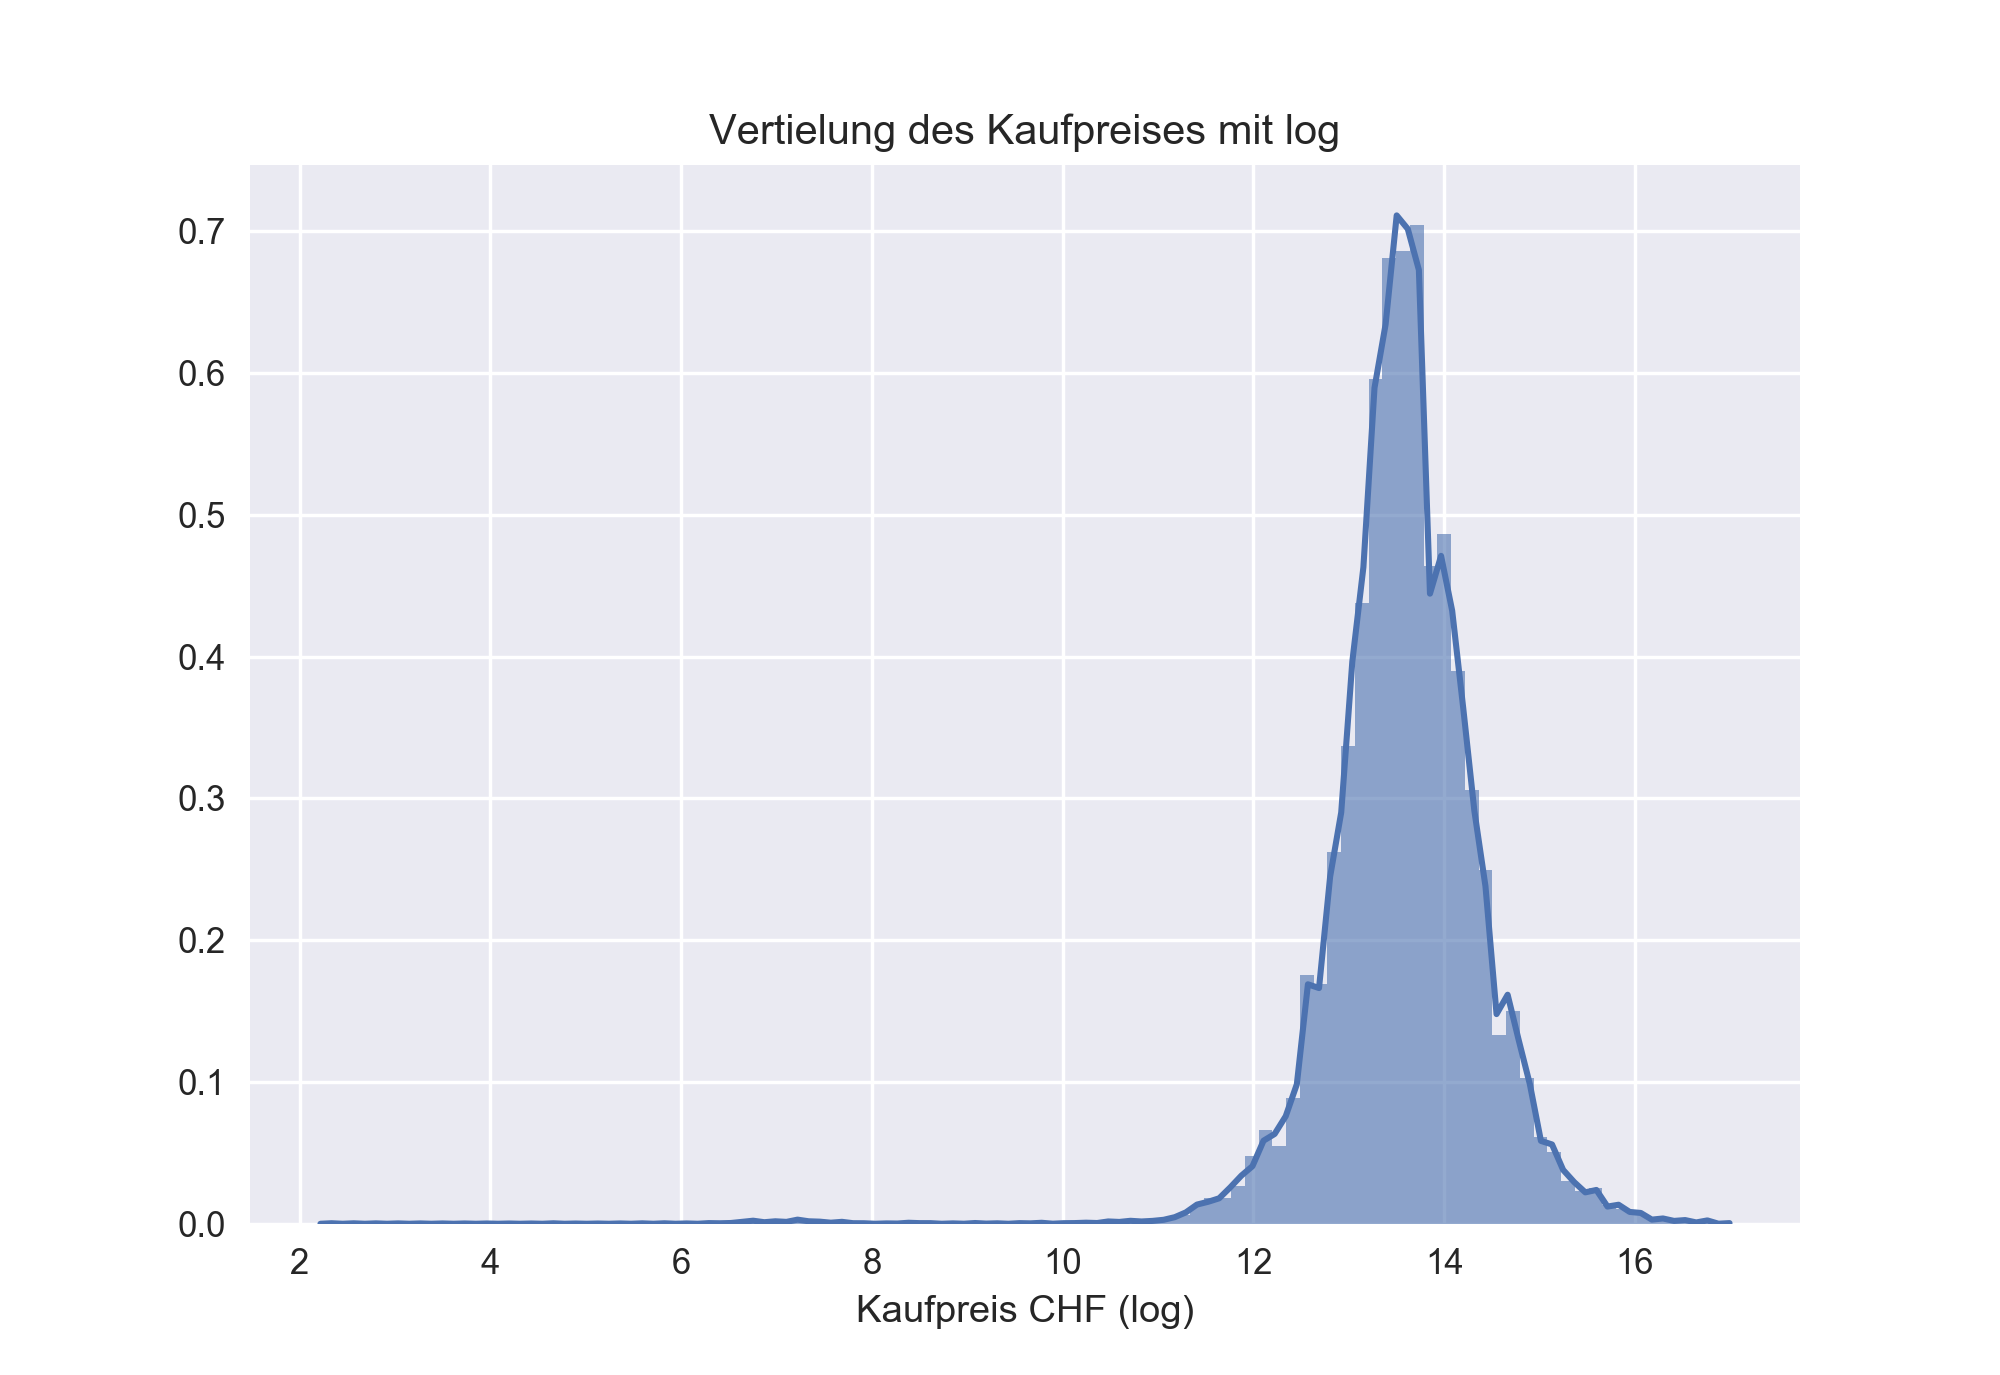
\includegraphics[width=\linewidth]{images/Verteilung_des_kauf_preises_log.png}
  \caption[Verteilung des Log(Preises)]{Verteilung des Log(Preises)}
  \label{fig:price_log}
\end{subfigure}
\caption[Kaufpreis analyse: Verteilung]{Kaufpreis analyse: Verteilung}
\label{fig:price}
\end{figure}
%
\begin{table*}[ht]
\centering
\ra{1.3}
\resizebox{\textwidth}{!}{
\begin{tabular}{@{}lrrrrr@{}}
\toprule
 & Min & Max & Durchschnitt & Median & Standardabweichung\\
\midrule
Preis: Haus & 10 & 20'000'000 & 1'281'735 & 920'000 & 1'309'085\\
Preis: Wohnung & 10 & 20'000'000 & 891’479 & 690’000 & 786’047\\
Pries: Alle & 10 & 20’000'000 & 1’059’503 & 790’000 & 1’066’372\\
\bottomrule
\end{tabular}}
\caption{Fehlermodelle mit Formelen}
\label{tab:error_models}
\end{table*}
%
\subsubsection{Numerische Features}
Bis auf die Lärmbelastung wurden alle numerischen Features von Inseraten gesammelt.\\
Abbildung \ref{fig:num_features} zeigt einen Teil dieser Features in Verbindung zum Kaufpreis. Dabei ist ersichtlich, dass die Wohnfläche, Kubatur und Anzahl Zimmer eine linear ähnliche Abhängigkeit haben. Beim Rest ist eher unklar, wie sie zum Preis stehen.\\[2ex]
%
\begin{figure}[h!]
\centering
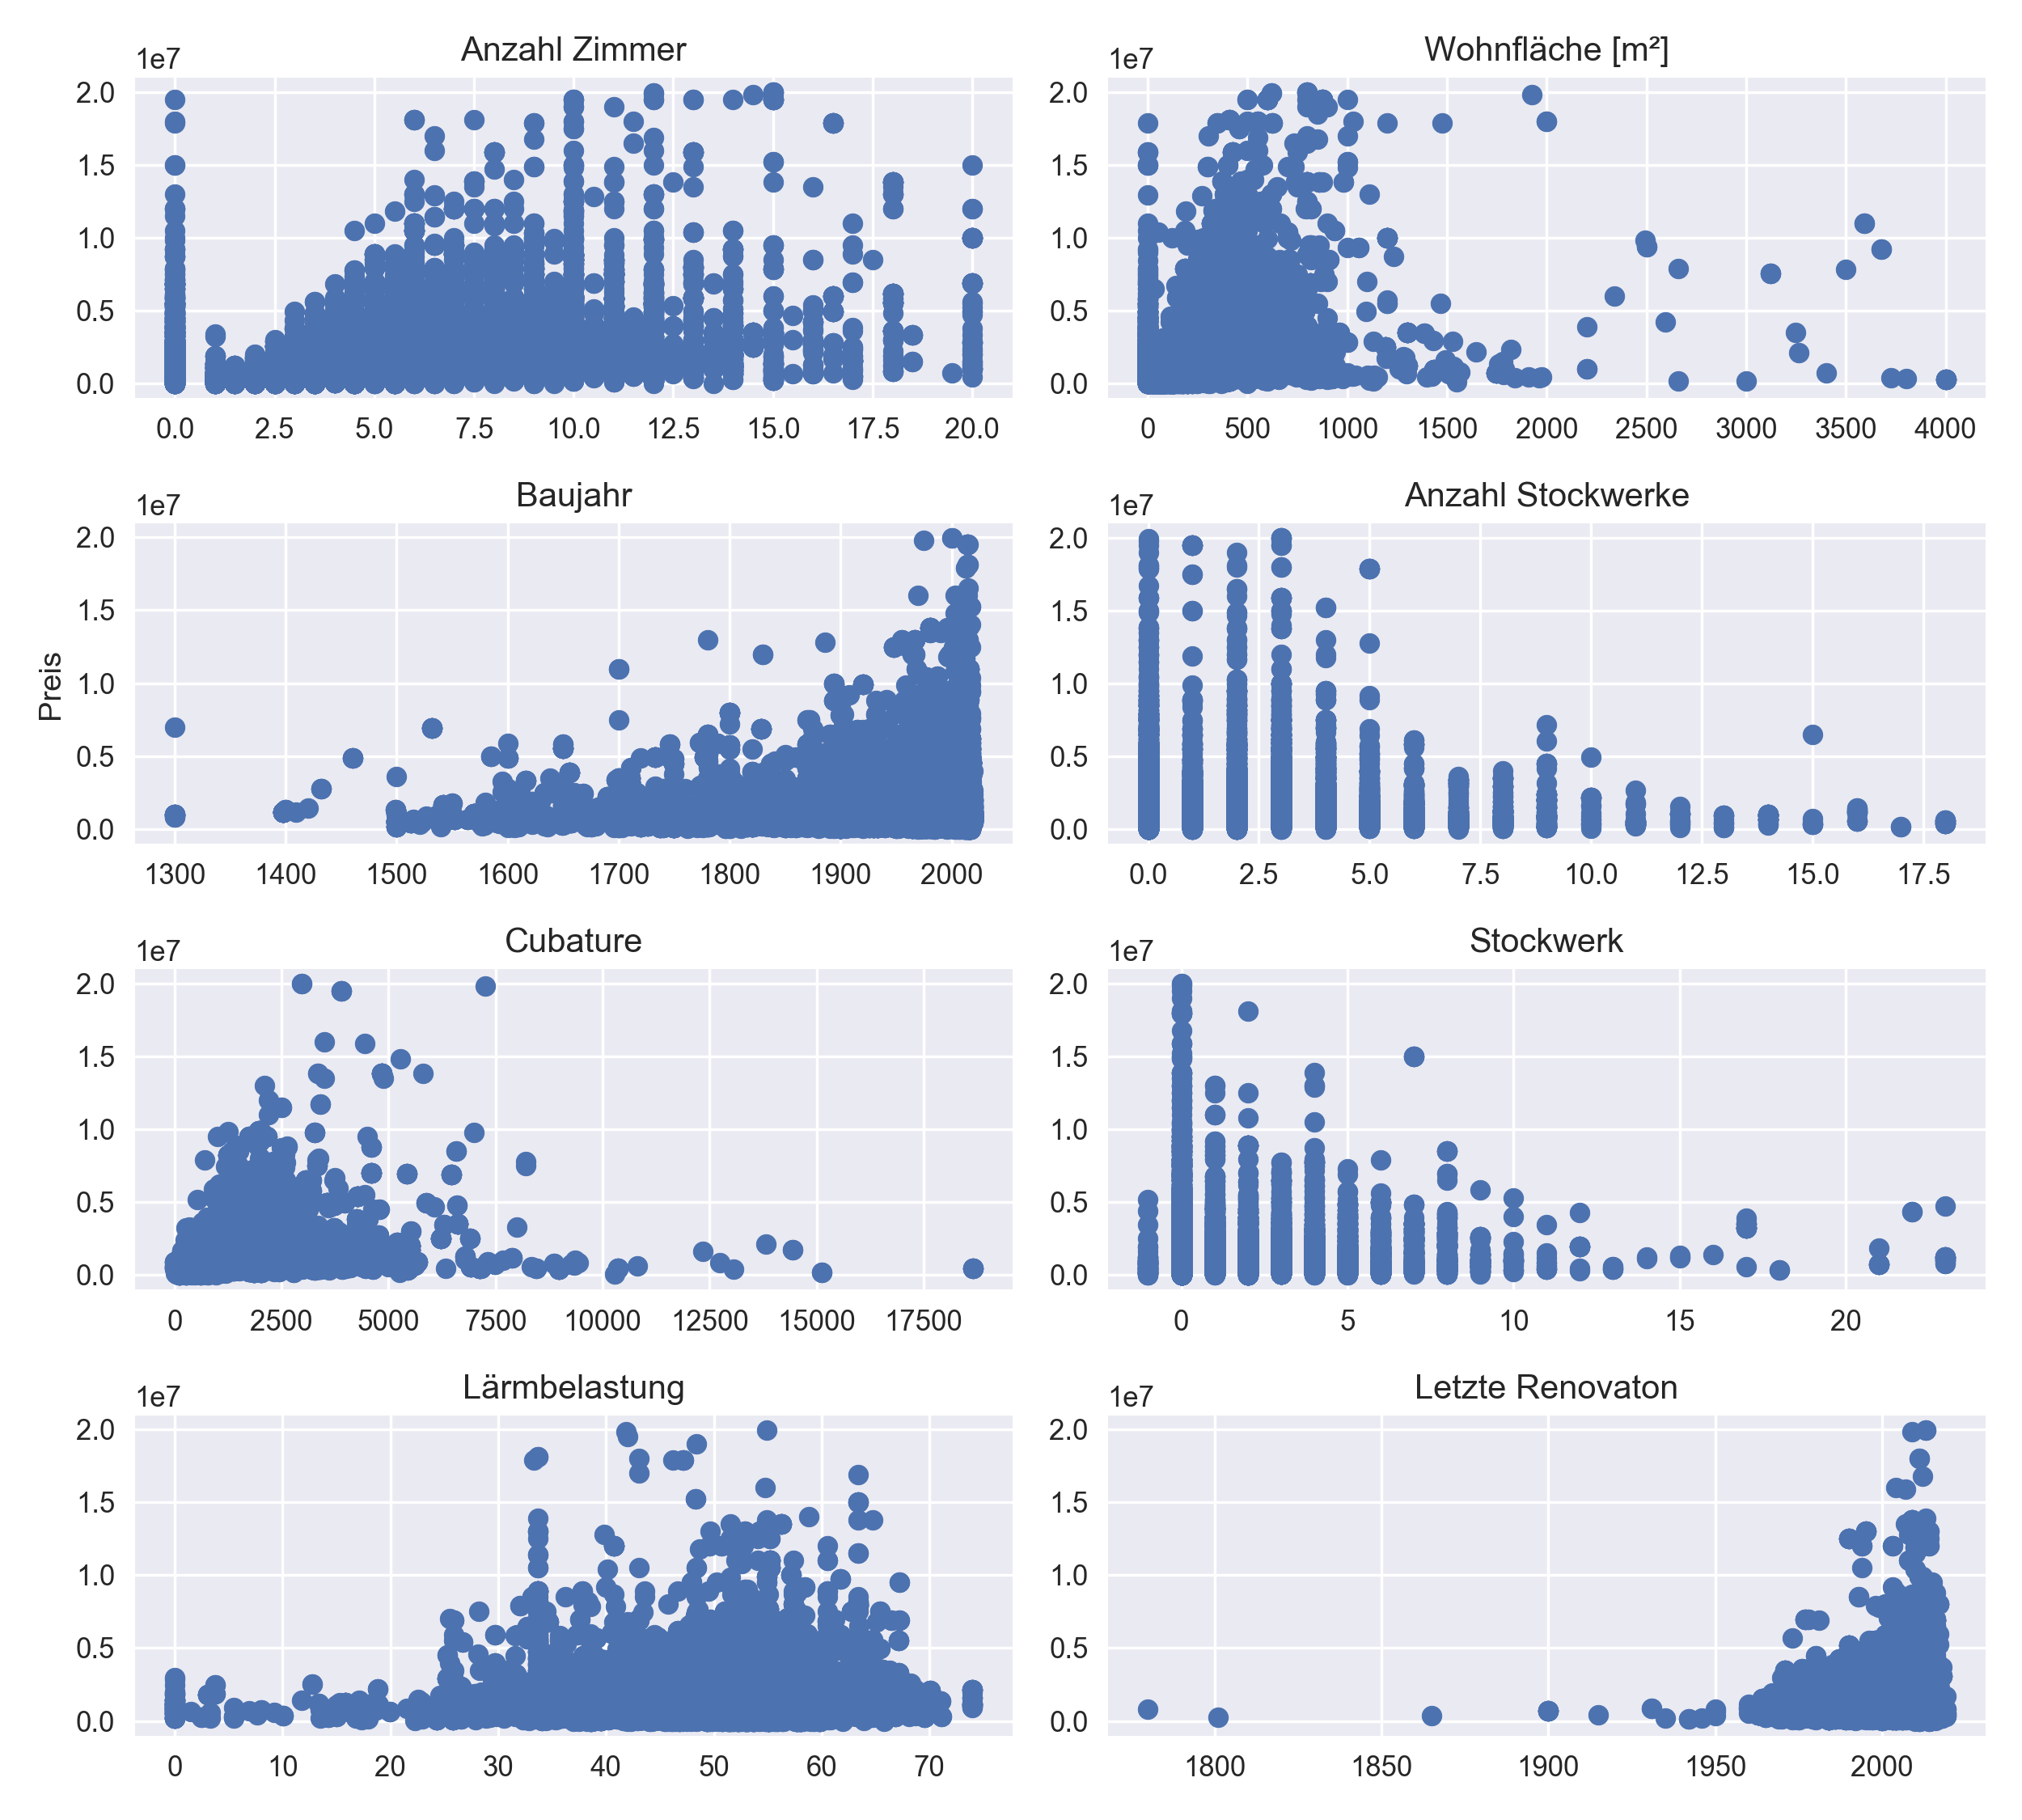
\includegraphics[width=0.9\textwidth]{images/Vergleich_zum_preis.png}
\caption[Nummerische Feature im Vergleich zum Preis]{Nummerische Feature im Vergleich zum Preis}%
\label{fig:num_features}
\end{figure}
\newline
%
Tabelle \ref{tab:num_features} zeigt die statistischen Werte für die numerischen Features. Die gesammelten Kennwerte sehen plausibel aus und decken sich zum Teil mit den Daten vom Bundesamt für Statistik\footnote{https://www.bfs.admin.ch/bfs/de/home/statistiken/bau-wohnungswesen.html}.\\
Auffallend ist, dass der Durchschnitt und der Median bei vielen Features sehr nahe beieinander liegen. Somit gleicht die Verteilung einer Normalverteilung.\\
Einzig störend sind die 0-Werte bei den Features Anzahl Zimmer und Fläche. Diese sollte wenn möglich weitgehend herausgefiltert werden.\\[2ex]
%
\begin{table*}[ht]
\centering
\ra{1.3}
\resizebox{\textwidth}{!}{
\begin{tabular}{@{}lrrrrr@{}}
\toprule
 & Min & Max & Durchschnitt & Median & Standardabweichung\\
\midrule
Anz. Zimmer & 0& 20 & 4.84 & 4.5 & 1.9\\
Fläche & 0 & 4’000 & 143.08 & 130 & 101.924\\
Baujahr & 1300 & 2019 & 1988 & 2006 & 51.52\\
Anz. Stockwerke & 0 & 18 & 1.8 & 2 & 1.747\\
Kubatur & 1 & 18649 & 1059.74 & 867 & 838.419\\
Stockwerk & -1 & 23 & 1.25 & 1 & 1.57\\
Lärmbelastung & 0 & 73.99 & 48.8 & 49.35 & 6.85\\
Letzte Renovation & 1780 & 2019 & 2009 & 2012 & 9.09\\
\bottomrule
\end{tabular}}
\caption{Statistische Werte der nummerischen Features}
\label{tab:num_features}
\end{table*}
%
Abbildung \ref{fig:heatmap} zeigt eine Heatmap der einzelnen Features. Sie zeigt, welche Features stark untereinander korrelieren. Folglich demonstriert sie von welchen Features der Preis abhängig ist. Somit sollte wenn möglich alle Features, die eine hohe Korrelation mit dem Kaufpreis besitzen, ins Modell miteinbezogen werden.
%
\begin{figure}[h!]
\centering
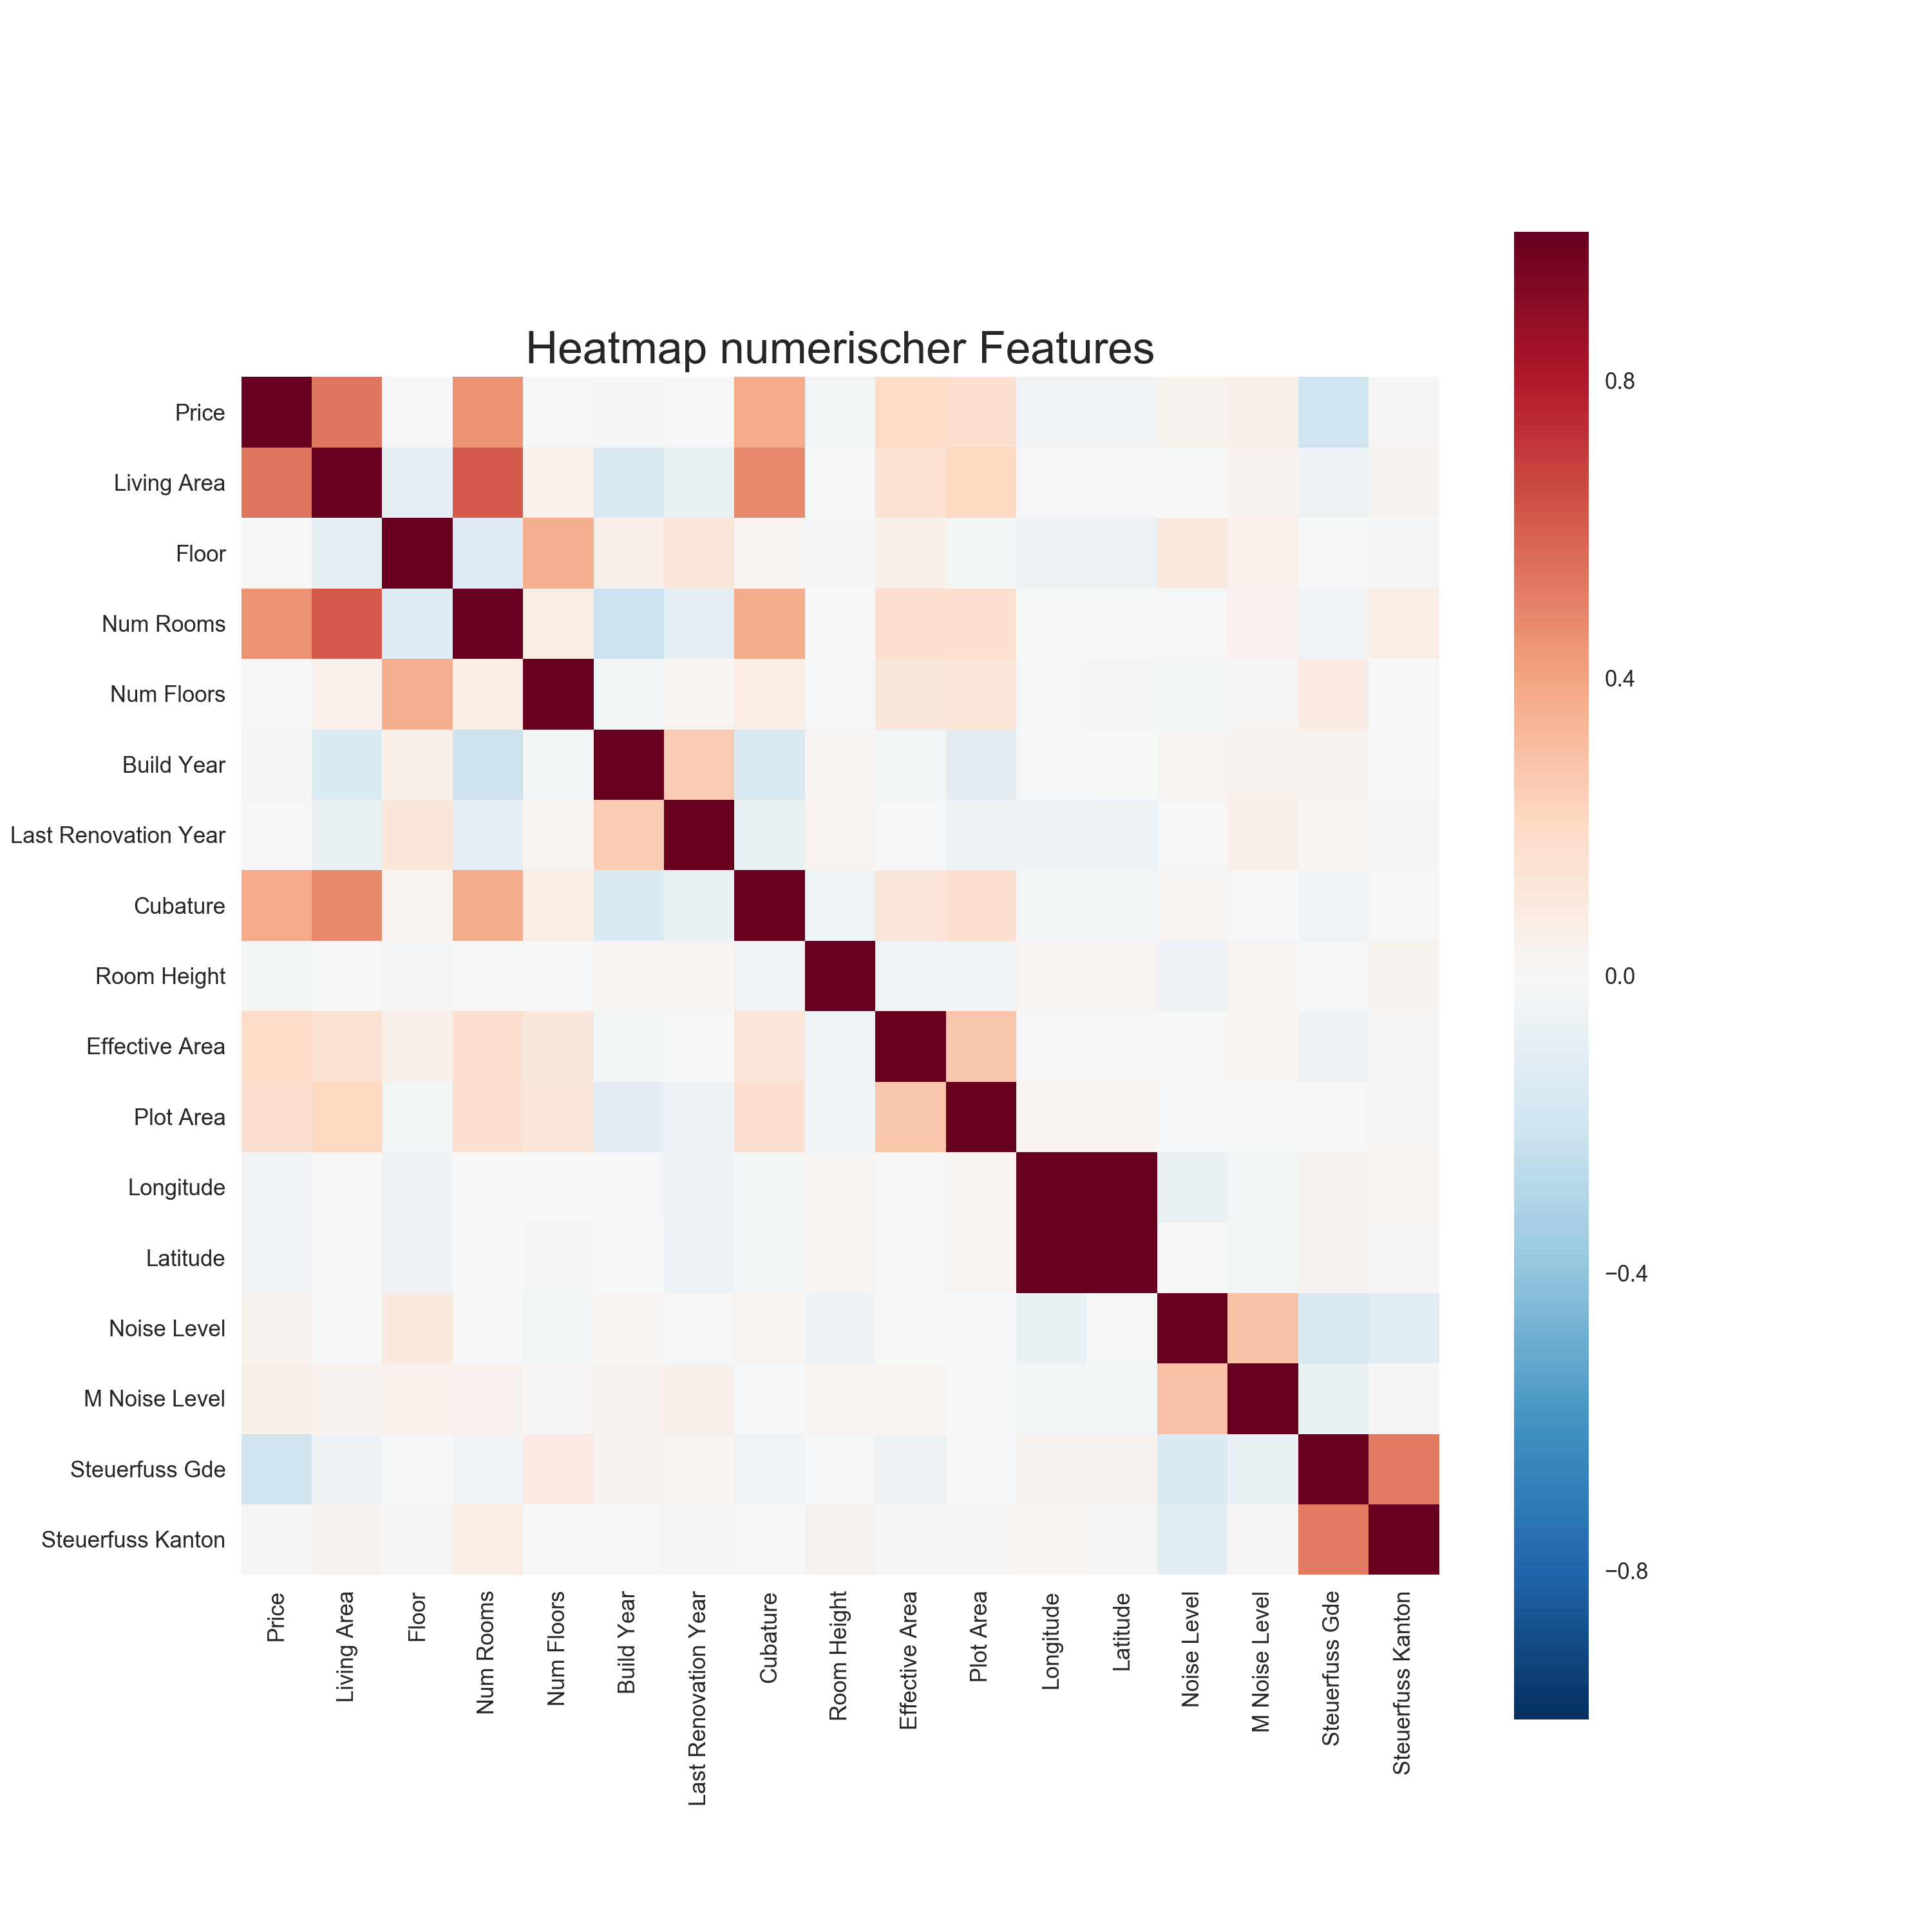
\includegraphics[width=0.9\textwidth]{images/Heatmap_numerical.png}
\caption[Heatmap der nummerischen Features]{Heatmap der nummerischen Features}%
\label{fig:heatmap}
\end{figure}
\newline
%
\subsubsection{Kategorische Features}
Bei den Kategorischen Features handelt es sich vor allem um ortsbezogene Features. Viele davon beschreiben die Region, indem sich die Immobilie befindet.\\
Insgesamt wurden 35 kategorische Features verwendet. Eine Analyse der ortsbezogenen Features mit dem Kaufpreis ergab keine unerwarteten Ergebnisse. So zeigt sich, dass der Kanton Genf die teuersten Immobilien in der Schweiz besitzt, gefolgt von Zug. Abbildung \ref{fig:cantons}.
Auch wurde ersichtlich, dass städtische Immobilien im Schnitt teurer sind als auf dem Land, beziehungsweise je urbaner die Region, desto teurer der Immobilienpreis. Weiter ist ersichtlich, dass  ein Haus im Schnitt mehr kostet als eine Wohnung.\\[2ex]
\begin{figure}[ht]
\centering
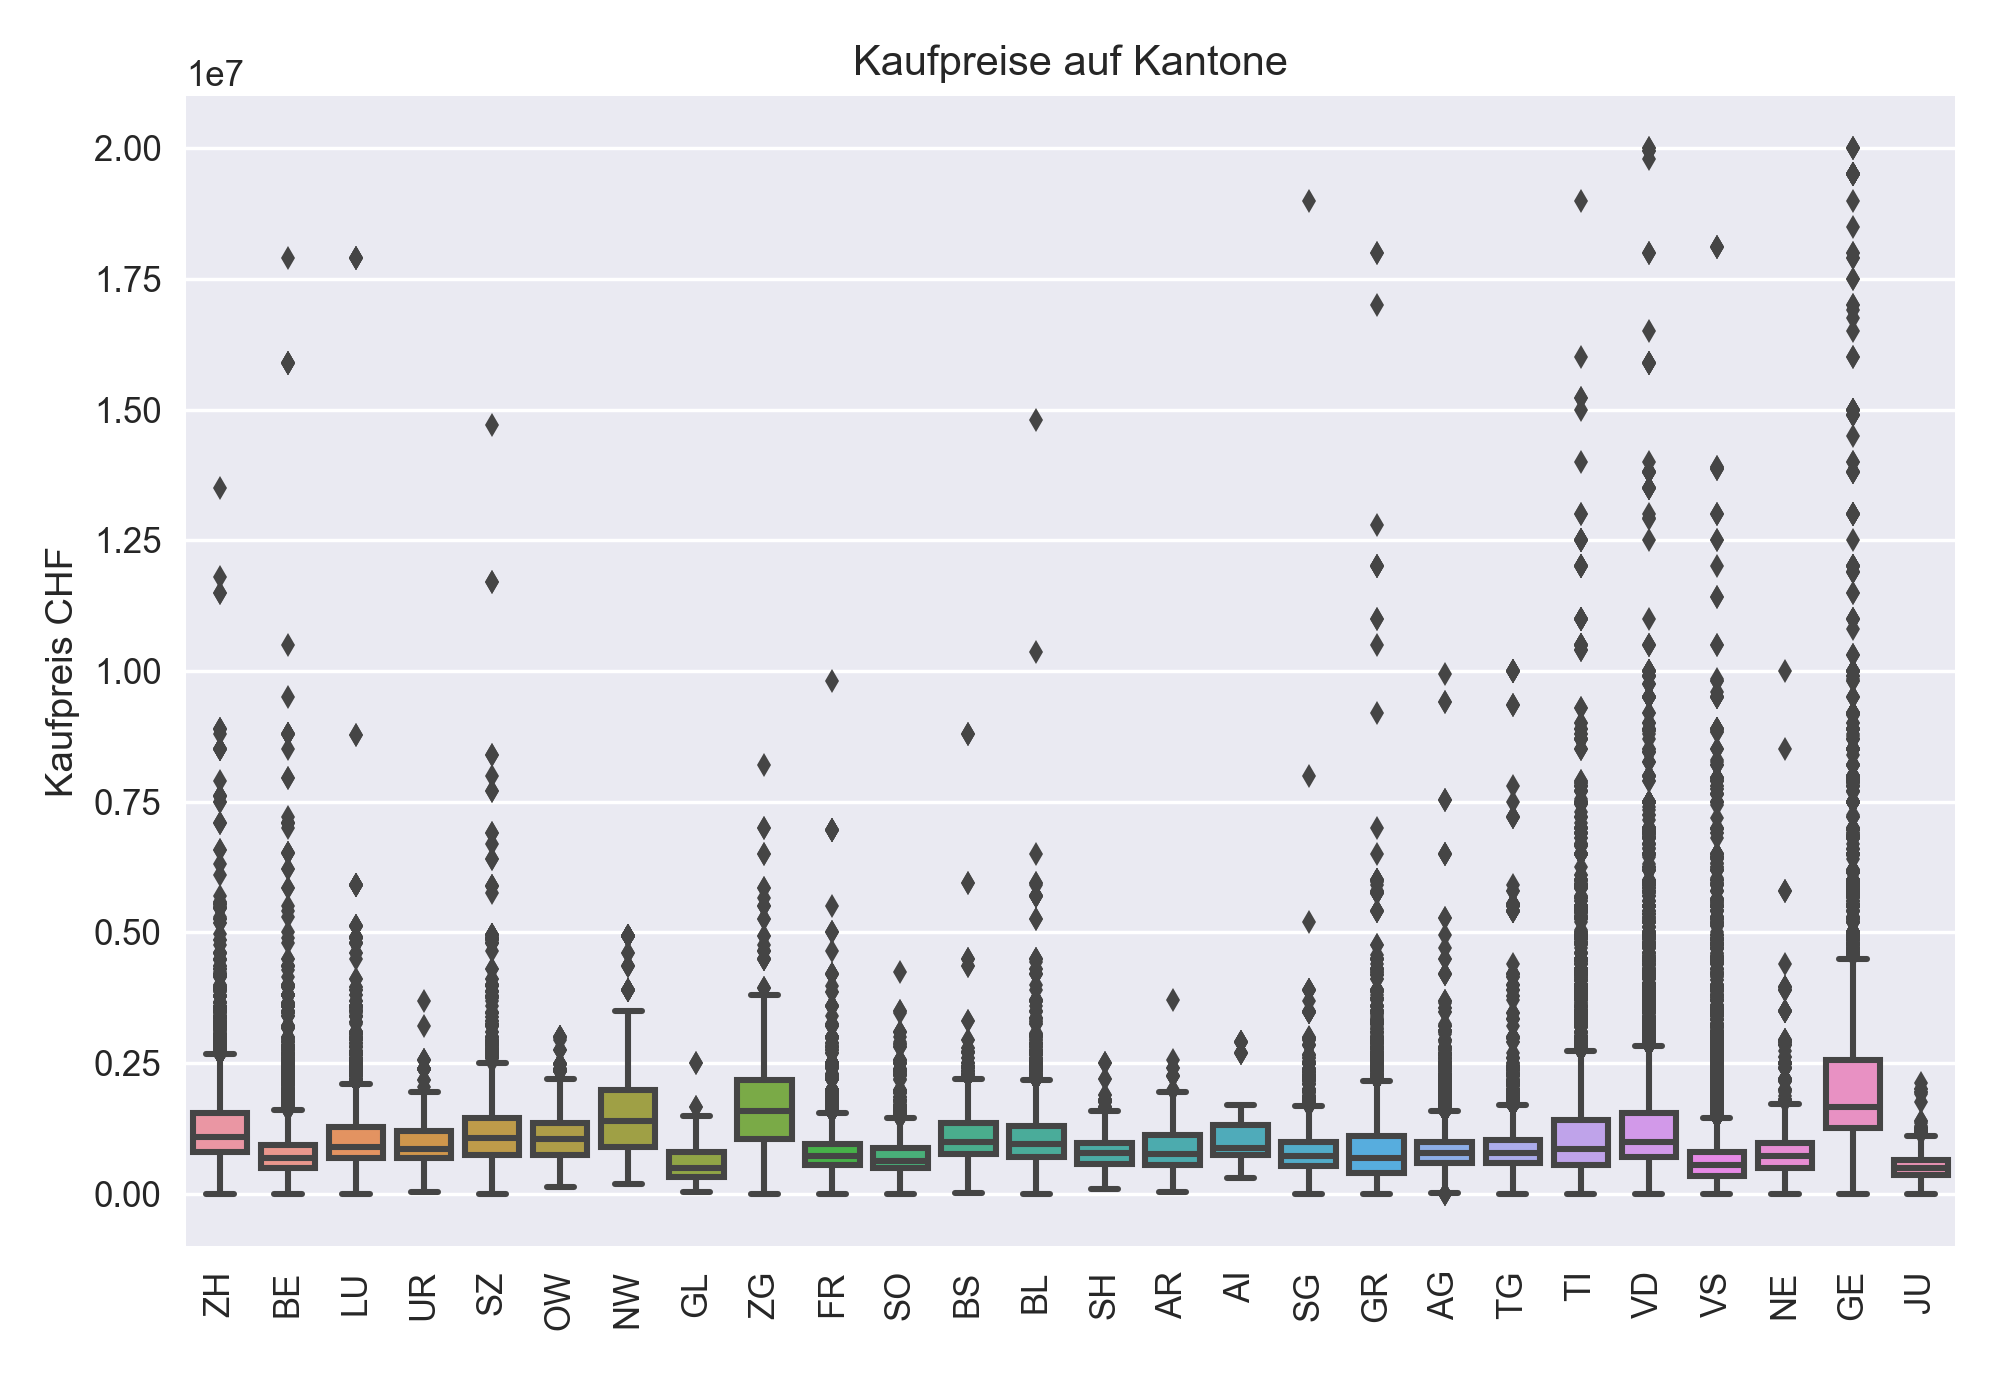
\includegraphics[width=\textwidth]{images/boxPlot_cantons.png}
\caption[Kaufpreis auf Kantonte aufgeteilt]{Kaufpreis auf Kantonte aufgeteilt}%
\label{fig:cantons}
\end{figure}
\newline
%
\textbf{Beschreibung / Charakteristik}
Weitere charakteristische Features stammen aus der Beschreibung und Merkmal analyse. Die 50 häufigsten vorkommenden Wörter die in unserem Datensatz vorkommen, werden in Abbildung \ref{fig:tags} gezeigt. 
\begin{figure}[ht]
\centering
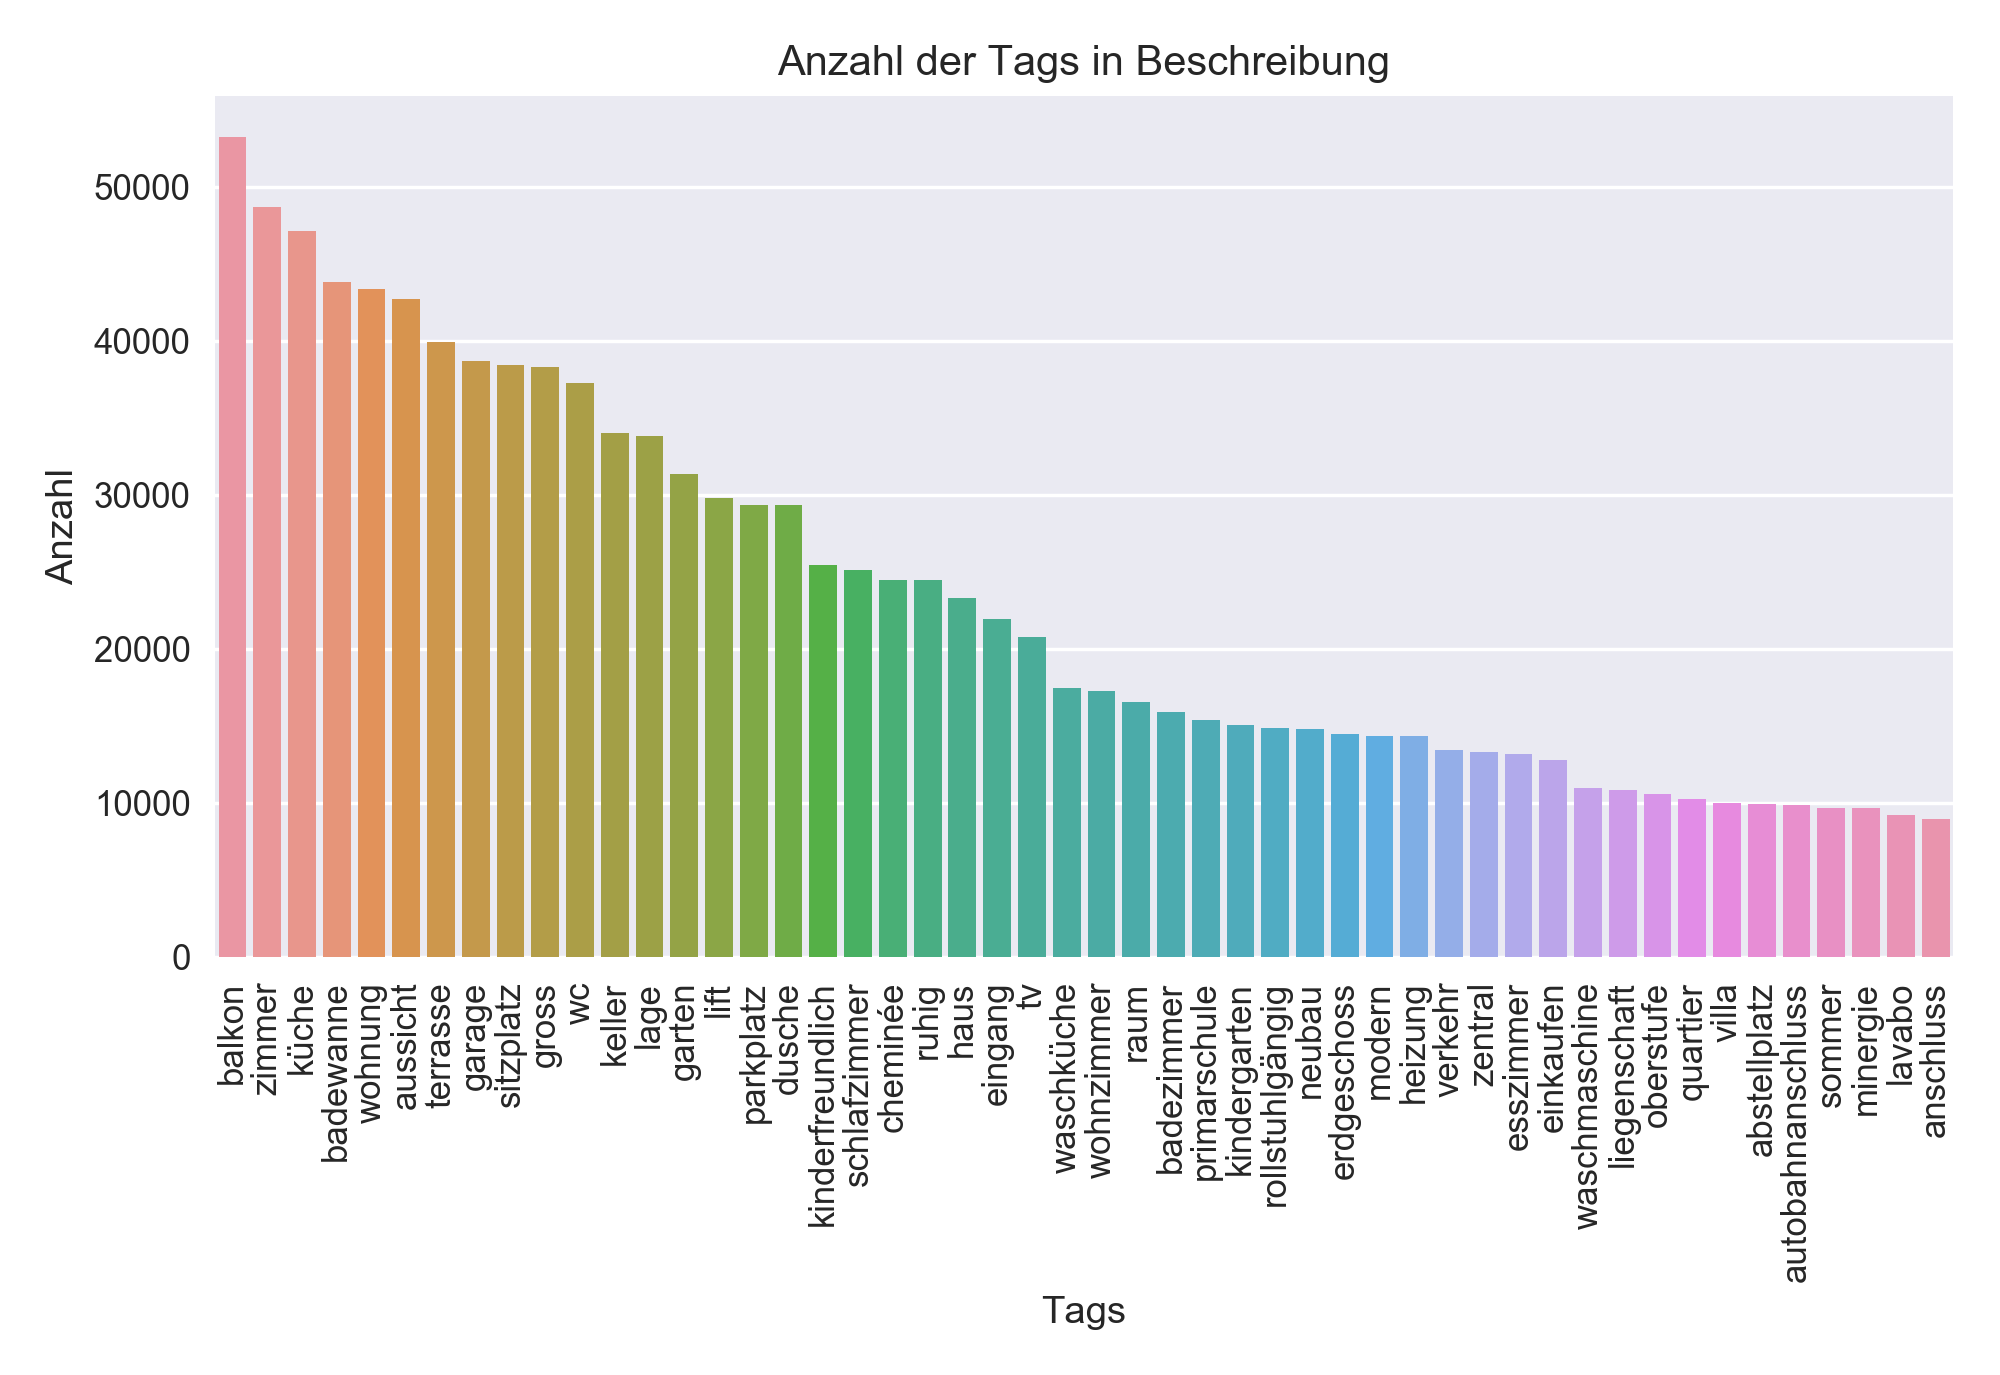
\includegraphics[width=\textwidth]{images/tags.png}
\caption[Häufigkeit der gefundenen Tags]{Häufigkeit der gefundenen Tags}%
\label{fig:tags}
\end{figure}
\newline
%
\subsection{Machine Learning}
Insgesamt haben wir neun verschiedene Machine Learning Algorithmen untersucht. Um eine faire Bewertung zu bekommen, bekamen alle Algorithmen die gleichen Datensätze zum Trainieren wie auch zum Testen. So wurde verhindert, dass ein Algorithmus anhand eines guten Datensatzes eine bessere Performance erzielte.\\[2ex]
%
Damit wir unsere gesammelten Daten für die Algorithmen verwenden können, müssen diese, wenn nötig, richtig transformiert werden. Dafür wird Feature Engineering angewendet, das nach und nach erweitert und verbessert wird.\\[2ex]
%
Als Basis für unsere Feature Engineering Pipeline transformieren wir unseren kategorischen Features mit Hilfe einer One-Hot-Encoding in binäre Features um. So konnten aus 35 Features über 2000 Features gewonnen werden.\\
Es ist nicht möglich alle gesammelten Features zu verwenden. Der Grund ist, dass gewisse Features nur bei wenigen Inseraten angegeben wurden. Wie im vorherigen Kapitel gezeigt, sind dies die Features Kubatur, Raumhöhe, effektive Fläche, Grundstücksfläche, Anzahl Stockwerke, Stockwerk und Renovationsjahr.\\
Als letzter Schritt werden die Inserate gelöscht, die keinen Eintrag bei einem verwendeten Feature besitzen oder doppelt vorkommen. Verwendet werden schlussendlich: Wohnfläche, Anzahl Zimmer, Baujahr Renovationsjahr, die Beschreibung und die Merkmale.\\[2ex]

Für die Auswertung der Algorithmen starten wir mit den Regressions Algorithmen. Hierfür verwenden wir: Lineare Regression, Ridge und der Lasso Algorithmus. Die Ergebnisse werden in Tabelle() angezeigt.


